\section{Flexible OS approaches}

CubicleOS~\cite{sartakov2021cubicleos}:
\begin{itemize}
    \item[]Identified Problem: 
    \item Library OSes and in particular the unikernels build form them are cool, but lack isolation among components after the kernels are compiled
    \item Microkernel based OSes on the other hand provide strong isolation piping everything through IPC calls. This means programmers have to tailor their component APIs to the communication mechanism of the respective microkernel. This also entails minimizing interaction as the frequent context switches degrade performance and that calls and transmitted data have to be adapted (e.g. any data passed to a cross service invocation has to be serializable). 
    \item The authors argue, that library OSes impose a particular burden on developers because they require adaptation of every third party component used. \means \textbf{This is a point for us. However, again ...we do not compile everything, but just the composition layer. So how do we make sure, that below this layer there is no interaction with the system that is written in traditional/monolith way and will not work on M$^3$?}
    \item implemented based on Unikraft library OS
    \item[] What is it?
    \item Cubicle consists of 1) a build tool 2) a trusted binary loader (for the user space Unikraft binaries?) 3) a trusted run-time using Intel MPK and Cublicles custom isolation-communication abstractions 4) an extension to MPK to verify control flow integrity
    \item[] How does it work? :
    \item Core abstractions are: \textit{cubicles}\means isolation for components (not sure if this would be nodes in our graph), \textit{windows}\means opening a \textit{window} with a data structure makes the data available for other cubicles without copying \question{How is sharing implemented?} after usage the \textit{window} is explicitly closed again  \question{What if it's not closed ... by accident?!} and \textit{ cross-cubicle calls} are an abstraction obviously for function calls designed to preserve control flow integrity and interface integrity (i.e. only 'public functions are public')
    \item The developer basically uses the windows in his code as shown in Figure ... taken from the original publication 
\end{itemize}
\begin{figure}[H]
    %\centering
    \begin{subfigure}[b]{0.45\textwidth}
         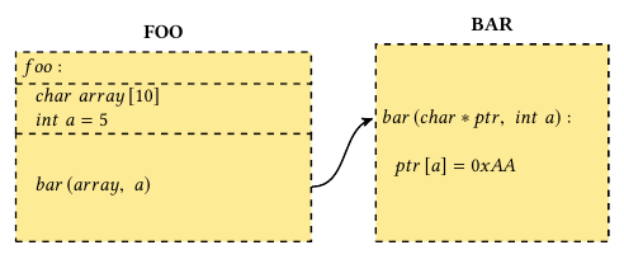
\includegraphics[width=\textwidth]{figures/cubicle_example_original.png}
         \caption{Original code of application FOO calling library BAR}
         \label{cubicleOriginal}
     \end{subfigure}
     \hfill
     \begin{subfigure}[b]{0.45\textwidth}
         %\centering
         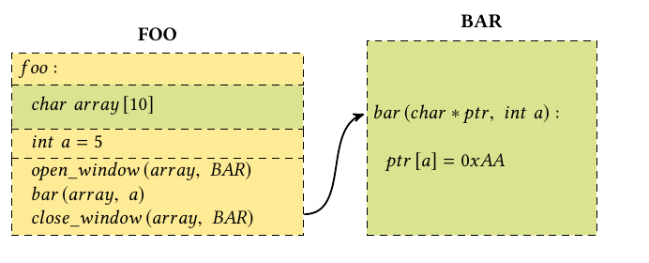
\includegraphics[width=\textwidth]{figures/cubicle_example_windows.png}
         \caption{Annotated code using Cubicles \textit{windows} to share memory after compilation}
         \label{cubicleWindow}
     \end{subfigure}
    \caption{To use Cubicle the developer basically needs to surround calls to other components, in this case BAR with \textit{windows}. Cubicle will derive isolated components and their (legitimate) interaction}
    \label{fig:CubicleAPI}
    \end{figure}

FlexOS~\cite{lefeuvre2021flexos} 
\begin{itemize}
    \item FlexOS is build on the ideas of library operating systems, in particular on the idea that 'everything is a library'. 
    \item This includes (micro)kernel components the system uses. 
    \item It is based on the Unikraft~\cite{kuenzer2021unikraft} library OS.
    \item FlexOS consists of a toolchain, a set of adapted libraries for all kinds of system/kernel functions (boot, networking, device drivers, memory access) and applications (e.g. nginx, redis, sqlite ...) and a set of supported 'Isolation Backends'. 
    \item Users provide the code for their application and a configuration specifying the libraries and backend to use and FlexOs will produce a custom, single-address space, single purpose OS for the compiled appliance.
    \item We do two things at the same time i) We isolate parts of the code from each other by extracting independent process steps from the composition code (build a DFG) and ii) We introduce backend specific communication mechanisms among the separated components. 
    \item FlexOS does only of this. 
    \item In particular, in the adapted libraries shared memory constructs as well as calls among different compartments (libraries) are marked with FlexOS specific placeholders. In the compilation process, the FlexOS toolchain replaces those placeholders with appropriate primitives for the selected 'Isolation Backend'. 
    \item \todo[inline]{At least the mechanism of keeping function calls abstract and making them concrete during compilation corresponds to the concrete implementation of channels in the backend. TODO: How exactly is shared state translated?}
\end{itemize}

\section{Compiling stateful imperative to Data Flow}
"Making State Explicit for Imperative Big Data Processing
"~\cite{fernandez2014making}:
\begin{itemize}
    \item identified problem: support arbitrary (Java) state in BigData (with high scalability) and recover state upon failure
    \item approach: infer dataflow and 'types of state access' to derive a 'stateful dataflow graph'(SDG)
    \item they explicitly focus on 'large states', where distribution of such state to several nodes is desirable both for performance/(storage/compute) capacity and for recovery after failure 
    \item SGD: "cyclic graph of pipelined data-parallel tasks, which exe-
cute on different nodes and access local in-memory state" \means no explicit scheduling
\item to identify 'partial' and 'partitioned' stateful objects, they require annotations from the programmer
\end{itemize}

"DFGenTool: A Dataflow Graph Generation Tool for Coarse Grain Reconfigurable Architectures "~\cite{mukherjee2017dfgentool}
\begin{itemize}
    \item based on LLVMIR
\end{itemize}